\clearpage

\subsection{Opaque without Survivability}\label{heuristic_Opaque_Survivability}
\begin{tcolorbox}	
\begin{tabular}{p{2.75cm} p{0.2cm} p{10.5cm}} 	
\textbf{Student Name}  &:& Pedro Coelho    (March 01, 2018 - )\\
\textbf{Goal}          &:& Implement the Heuristic model for the opaque transport mode without survivability.
\end{tabular}
\end{tcolorbox}

\subsubsection{Model description}

\vspace{11pt}
In the opaque transport mode (link-by-link approach), the lightpath entering any intermediate node is necessarily terminated, i.e., there are performed OEO (optical-electrical-optical) conversions at every intermediate node since the origin to the destination node. These conversions are used for every wavelength at every node.

Contrary to the opaque with dedicated 1+1 protection technique, the opaque without survivability technique does not have a backup path, so if there is a network failure it is more likely to suffer large data losses, which consequently leads to higher network costs. However, the CAPEX will be significantly lower, because that not includes a secondary path that would increase several network elements.

For this model, after the creation of the matrices and the network topology, it is necessary to apply the routing and grooming algorithms created. For the "Logical Topology" algorithm, the user must insert "Opaque" in the "logicalTopology" value and for the "Grooming" algorithm, the user must insert "no" in the parameter value "protection".

At the end, the "Cost Report" algorithm will be applied to obtain the best CAPEX result for the network in question.

Firstly, in the opaque transport mode, the optical node cost is 0 because all the ports in the network are electrical. Consequently, to calculate the nodes' cost in this transport mode it only has to be considered the electrical nodes' cost:

\begin{itemize}
  \item $N_{OXC,n}$ = 0, \quad $\forall$ n
  \item $N_{EXC,n}$ = 1, \quad $\forall$ n that process traffic
\end{itemize}

As previously mentioned, equation \ref{EXC_pexc1_opaque_heuristic} refers to the number of long-reach ports of the electrical switch with bit-rate -1 in node $n$, $P_{exc,-1,n}$, i.e., the number of line ports of node $n$ which can be calculated as

\begin{equation}
P_{exc,-1,n} = \sum_{j=1}^{N} w_{nj}
\label{EXC_pexc1_opaque_heuristic}
\end{equation}

\vspace{11pt}
where $w_{nj}$ is the number of optical channels between node $n$ and node $j$.

\newpage
\vspace{11pt}
As previously mentioned, equation \ref{EXC_pexc2_opaque_heuristic} refers to the number of short-reach ports of the
electrical switch with bit-rate $c$ in node $n$, $P_{exc,c,n}$, i.e., the number of tributary ports with bit-rate $c$ in node $n$ which can be calculated as

\begin{equation}
P_{exc,c,n} = \sum_{d=1}^{N} D_{nd,c}
\label{EXC_pexc2_opaque_heuristic}
\end{equation}

\vspace{11pt}
where $D_{nd,c}$ are the client demands between nodes $n$ and $d$ with bit rate $c$.

\vspace{11pt}
In this case there is the following particularity:

\begin{itemize}
  \item When $n$=$j$, the value of client demands is always zero, i.e, $D_{nn,c}=0$.
\end{itemize}

\subsubsection{Result description}

It is already known all the necessary formulas to obtain the CAPEX value for the reference network \ref{Reference_Network_Topology}. As described in the subsection of the network traffic \ref{Reference_Network_Traffic}, it is necessary to obtain three different values of CAPEX for the low (0.5 Tbit/s), medium (5 Tbit/s) and high (10 Tbit/s) traffic. It is used a network software program called Net2Plan which can design the traffic matrices, create all the network topologies, simulate the algorithms into the network implemented in the programming software called Eclipse and analyze the results obtained.

In this chapter will be demonstrated the results by Vasco's heuristics from 2016. In each of the three traffic scenarios, it will be shown the network topologies followed by the table with the CAPEX value of the network.\\

\textbf{Low Traffic Scenario:}\\

In this scenario we have to take into account the traffic calculated in \ref{low_traffic_scenario}. In a first phase we will show the various existing topologies of the network. The first are the allowed topologies, physical and optical topology, the second are the logical topology for all ODUs and finally the resulting physical and optical topology.\\

\begin{figure}[H]
\centering
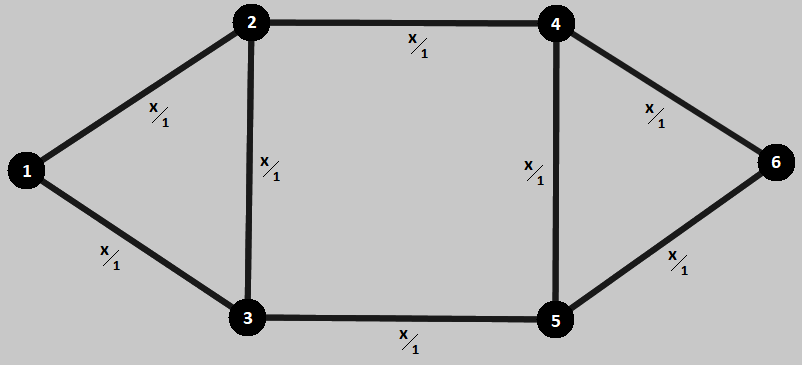
\includegraphics[width=13cm]{sdf/heuristic/figures/topologies/opaque_surv/low/allowed_physical_low}
\caption{Allowed Physical Topology.}
\label{allowed_physical_surv_ref_low_heuristic}
\end{figure}

\begin{figure}[H]
\centering
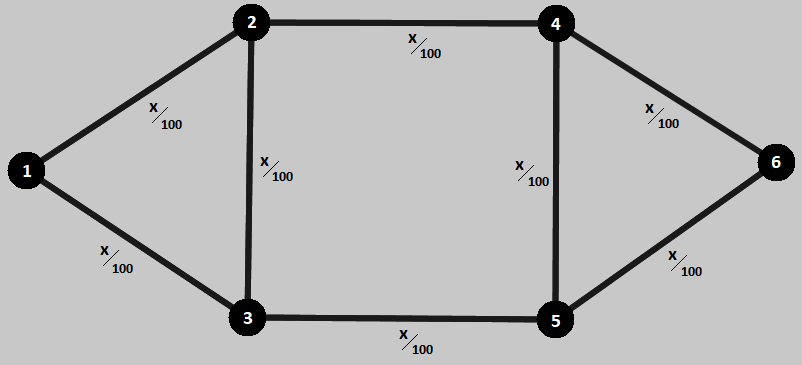
\includegraphics[width=13cm]{sdf/heuristic/figures/topologies/opaque_surv/low/allowed_optical_low}
\caption{Allowed Optical Topology.}
\label{allowed_optical_surv_ref_low_heuristic}
\end{figure}

\begin{figure}[H]
\centering
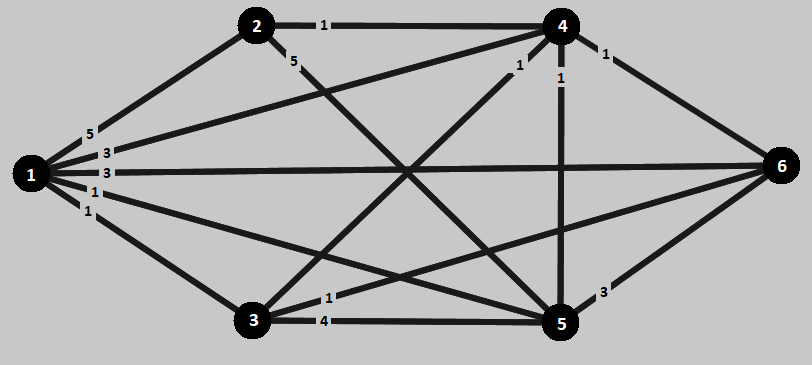
\includegraphics[width=13cm]{sdf/heuristic/figures/topologies/opaque_surv/low/logical_topology_odu0_low}
\caption{Logical Topology of ODU0.}
\label{logical_ODU0_surv_ref_low_heuristic}
\end{figure}

\begin{figure}[H]
\centering
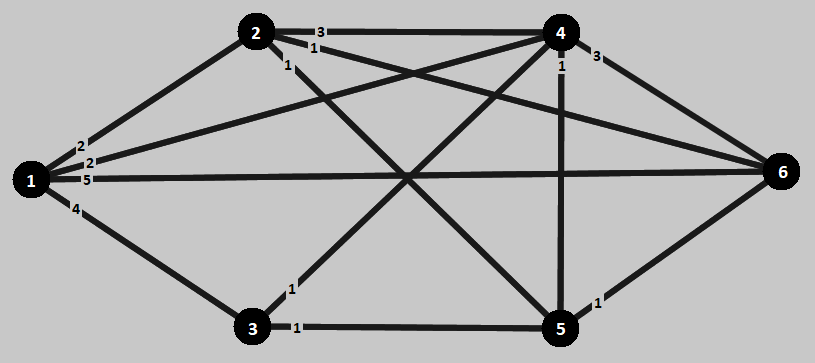
\includegraphics[width=13cm]{sdf/heuristic/figures/topologies/opaque_surv/low/logical_topology_odu1_low}
\caption{Logical Topology of ODU1.}
\label{logical_ODU1_surv_ref_low_heuristic}
\end{figure}

\begin{figure}[H]
\centering
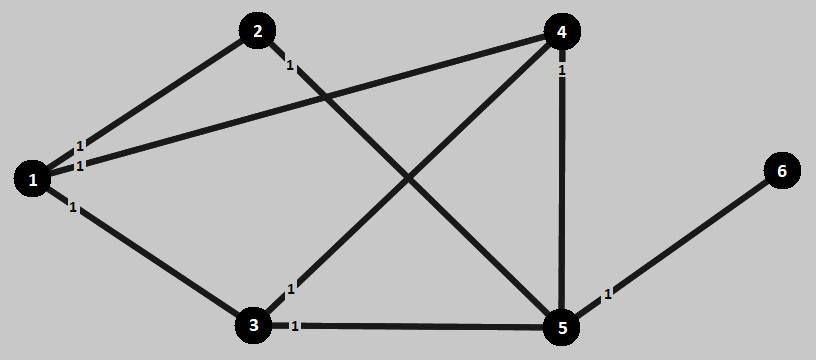
\includegraphics[width=13cm]{sdf/heuristic/figures/topologies/opaque_surv/low/logical_topology_odu2_low}
\caption{Logical Topology of ODU2.}
\label{logical_ODU2_surv_ref_low_heuristic}
\end{figure}

\begin{figure}[H]
\centering
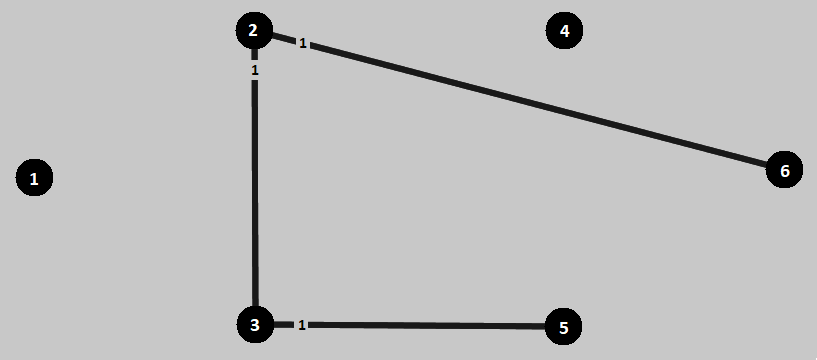
\includegraphics[width=13cm]{sdf/heuristic/figures/topologies/opaque_surv/low/logical_topology_odu3_low}
\caption{Logical Topology of ODU3.}
\label{logical_ODU3_surv_ref_low_heuristic}
\end{figure}

\begin{figure}[H]
\centering
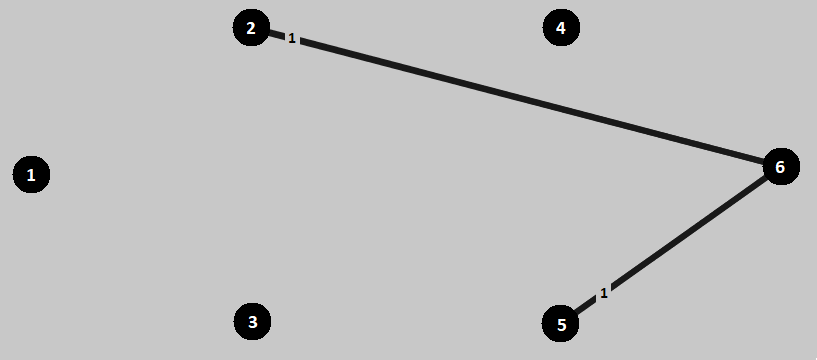
\includegraphics[width=13cm]{sdf/heuristic/figures/topologies/opaque_surv/low/logical_topology_odu4_low}
\caption{Logical Topology of ODU4.}
\label{logical_ODU4_surv_ref_low_heuristic}
\end{figure}

\begin{figure}[H]
\centering
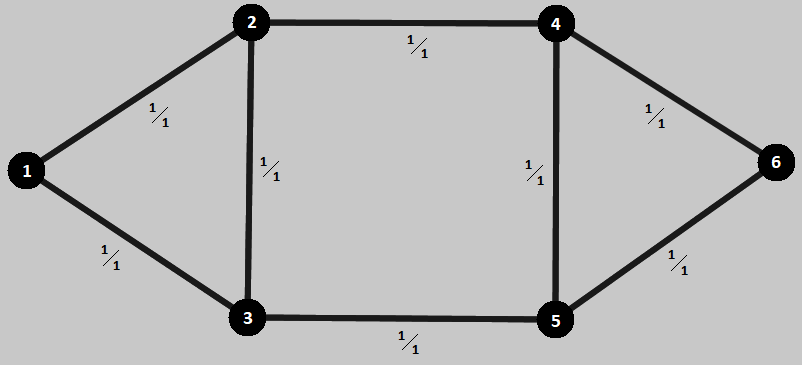
\includegraphics[width=13cm]{sdf/heuristic/figures/topologies/opaque_surv/low/physical_topology_low}
\caption{Physical Topology.}
\label{physical_topology_surv_ref_low_heuristic}
\end{figure}

Following all the steps mentioned in the \ref{net2plan_guide}, applying the routing and grooming heuristic algorithms in the Net2Plan software and using all the data referring to this scenario, the obtained result for the Vasco's heuristics can be consulted in the following table:

\begin{table}[H]
\centering
\begin{tabular}{|| c | c | c | c | c | c | c ||}
 \hline
 \multicolumn{7}{|| c ||}{CAPEX of the Network} \\
 \hline
 \hline
 \multicolumn{3}{|| c |}{ } & Quantity & Unit Price & Cost & Total \\
 \hline
 \multirow{3}{*}{Link Cost} & \multicolumn{2}{ c |}{OLTs} & 16 & 15 000 \euro & 240 000 \euro & \multirow{3}{*}{13 520 000 \euro} \\ \cline{2-6}
 & \multicolumn{2}{ c |}{100 Gb/s Transceivers} & 26 & 5 000 \euro/Gb/s & 13 000 000 \euro & \\ \cline{2-6}
 & \multicolumn{2}{ c |}{Amplifiers} & 70 & 4 000 \euro & 280 000 \euro & \\
 \hline
 \multirow{9}{*}{Node Cost} & \multirow{7}{*}{Electrical} & EXCs & 6 & 10 000 \euro & 60 000 \euro & \multirow{9}{*}{2 662 590 \euro} \\ \cline{3-6}
 & & ODU0 Ports & 60 & 8 \euro/Gb/s & 600 \euro & \\ \cline{3-6}
 & & ODU1 Ports & 50 & 6 \euro/Gb/s & 750 \euro & \\ \cline{3-6}
 & & ODU2 Ports & 16 & 3 \euro/Gb/s & 480 \euro & \\ \cline{3-6}
 & & ODU3 Ports & 6 & 1.5 \euro/Gb/s & 360 \euro & \\ \cline{3-6}
 & & ODU4 Ports & 4 & 1 \euro/Gb/s & 400 \euro & \\ \cline{3-6}
 & & Line Ports & 26 & 1 000 \euro/Gb/s & 2 600 000 \euro & \\ \cline{2-6}
 & \multirow{2}{*}{Optical} & OXCs & 0 & 20 000 \euro & 0 \euro & \\ \cline{3-6}
 & & Ports & 0 & 2 500 \euro/porto & 0 \euro & \\
 \hline
 \multicolumn{6}{|| c |}{Total Network Cost} & 16 182 590 \euro \\
\hline
\end{tabular}
\caption{Table with detailed description of CAPEX of Vasco's 2016 results.}
\label{scriptopaque_surv_ref_low_heuristic_Vasco}
\end{table}

Through the formulas mentioned below we can see how all the values of the quantity column were calculated.

\begin{table}[H]
\centering
\begin{tabular}{|| c | c ||}
 \hline
 OLTs: & \(\displaystyle 2 \sum_{i=1}^{N}\sum_{j=i+1}^{N} L_{ij} \) \\ \hline
 Transceivers: & \(\displaystyle 2 \sum_{i=1}^{N}\sum_{j=i+1}^{N} W_{ij} \) \\ \hline
 Amplifiers: & \(\displaystyle \sum_{i=1}^{N}\sum_{j=i+1}^{N} N^R_{ij} L_{ij} \) \\ \hline
 EXCs: & \(\displaystyle \sum_n^N N_{EXC,n} \) \\ \hline
 ODU0: & \(\displaystyle \sum_{o=1}^{N}\sum_{d=1}^{N} D_{od,0} \) \\ \hline
 ODU1: & \(\displaystyle \sum_{o=1}^{N}\sum_{d=1}^{N} D_{od,1} \) \\ \hline
 ODU2: & \(\displaystyle \sum_{o=1}^{N}\sum_{d=1}^{N} D_{od,2} \)\\ \hline
 ODU3: & \(\displaystyle \sum_{o=1}^{N}\sum_{d=1}^{N} D_{od,3} \) \\ \hline
 ODU4: & \(\displaystyle \sum_{o=1}^{N}\sum_{d=1}^{N} D_{od,4} \) \\ \hline
 Line: & \(\displaystyle \sum_{i=1}^{N}\sum_{j=1}^{N} W_{ij} \) \\ \hline
 OXCs: & As mentioned initially this result is always zero. \\ \hline
 Ports: & Does not exist for this case then it is equal to zero. \\
 \hline
 \end{tabular}
\caption{Table with description of calculation}
\label{formulas_opaque_surv_ref_low_heuristic}
\end{table}

\newpage
\textbf{Medium Traffic Scenario:}\\

In this scenario we have to take into account the traffic calculated in \ref{low_traffic_scenario}. In a first phase we will show the various existing topologies of the network. The first are the allowed topologies, physical and optical topology, the second are the logical topology for all ODUs and finally the resulting physical and optical topology.\\

\begin{figure}[H]
\centering
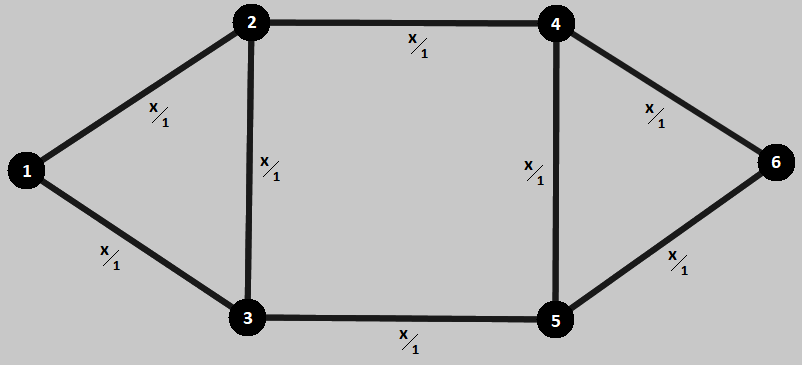
\includegraphics[width=13cm]{sdf/heuristic/figures/topologies/opaque_surv/medium/allowed_physical_medium}
\caption{Allowed Physical Topology.}
\label{allowed_physical_surv_ref_medium_heuristic}
\end{figure}

\begin{figure}[H]
\centering
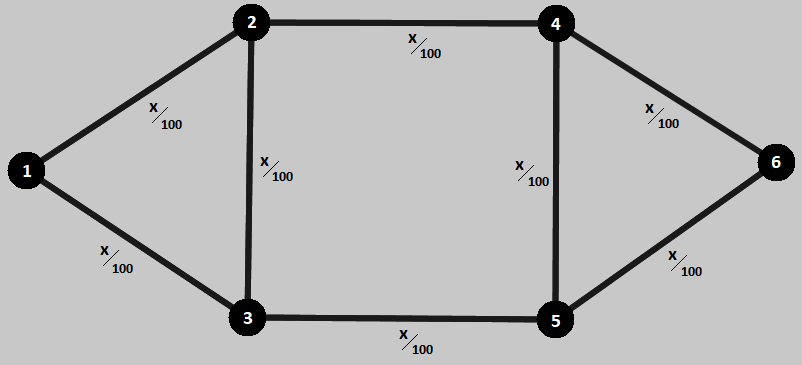
\includegraphics[width=13cm]{sdf/heuristic/figures/topologies/opaque_surv/medium/allowed_optical_medium}
\caption{Allowed Optical Topology.}
\label{allowed_optical_surv_ref_medium_heuristic}
\end{figure}

\begin{figure}[H]
\centering
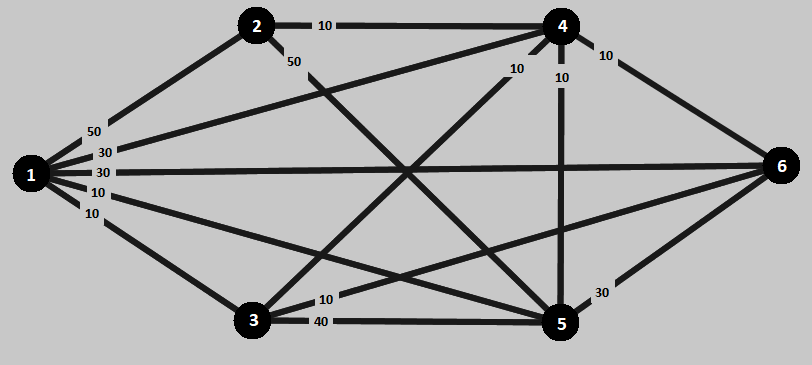
\includegraphics[width=13cm]{sdf/heuristic/figures/topologies/opaque_surv/medium/logical_topology_odu0_medium}
\caption{Logical Topology of ODU0.}
\label{logical_ODU0_surv_ref_medium_heuristic}
\end{figure}

\begin{figure}[H]
\centering
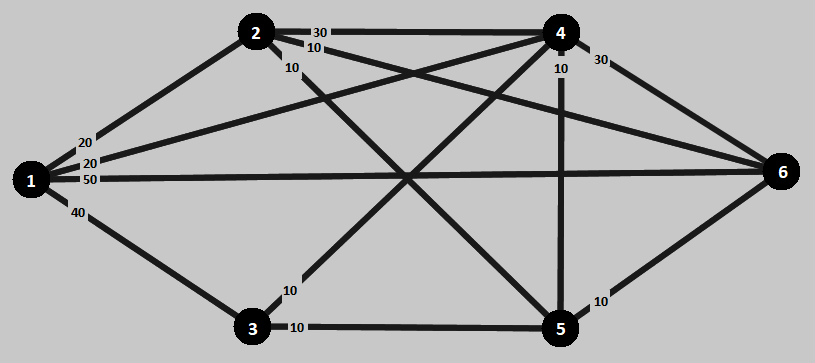
\includegraphics[width=13cm]{sdf/heuristic/figures/topologies/opaque_surv/medium/logical_topology_odu1_medium}
\caption{Logical Topology of ODU1.}
\label{logical_ODU1_surv_ref_medium_heuristic}
\end{figure}

\begin{figure}[H]
\centering
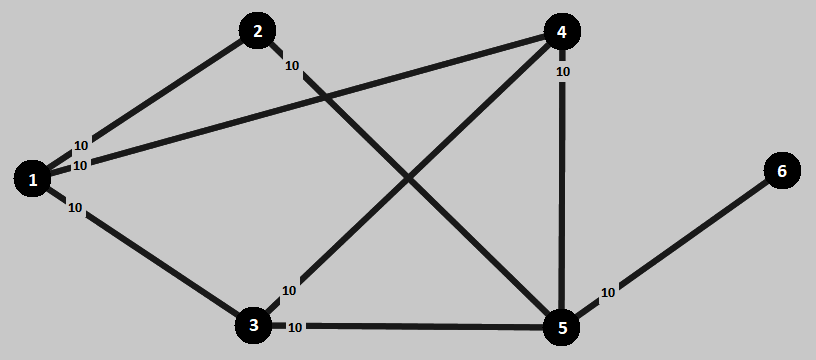
\includegraphics[width=13cm]{sdf/heuristic/figures/topologies/opaque_surv/medium/logical_topology_odu2_medium}
\caption{Logical Topology of ODU2.}
\label{logical_ODU2_surv_ref_medium_heuristic}
\end{figure}

\begin{figure}[H]
\centering
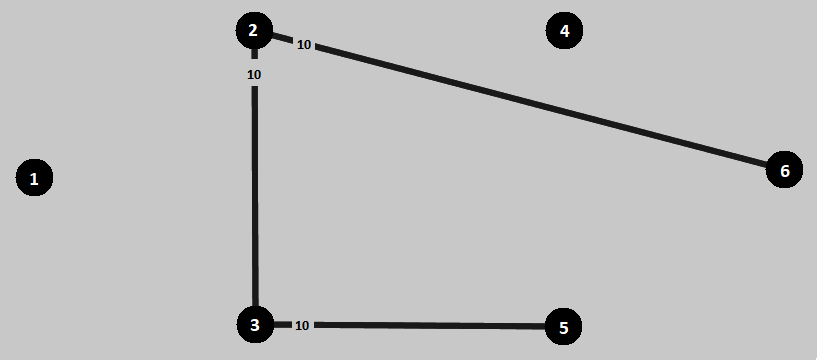
\includegraphics[width=13cm]{sdf/heuristic/figures/topologies/opaque_surv/medium/logical_topology_odu3_medium}
\caption{Logical Topology of ODU3.}
\label{logical_ODU3_surv_ref_medium_heuristic}
\end{figure}

\begin{figure}[H]
\centering
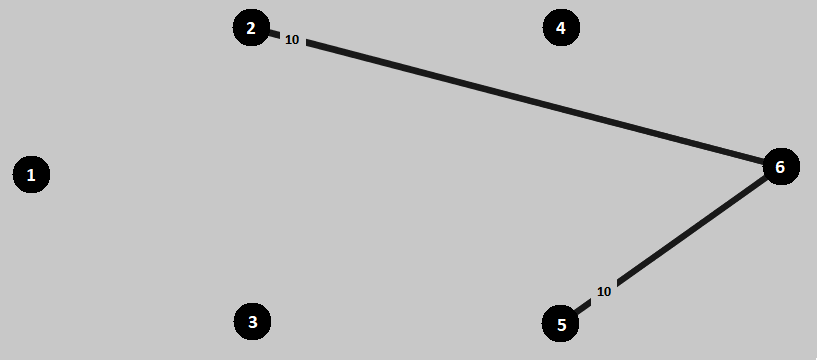
\includegraphics[width=13cm]{sdf/heuristic/figures/topologies/opaque_surv/medium/logical_topology_odu4_medium}
\caption{Logical Topology of ODU4.}
\label{logical_ODU4_surv_ref_medium_heuristic}
\end{figure}

\begin{figure}[H]
\centering
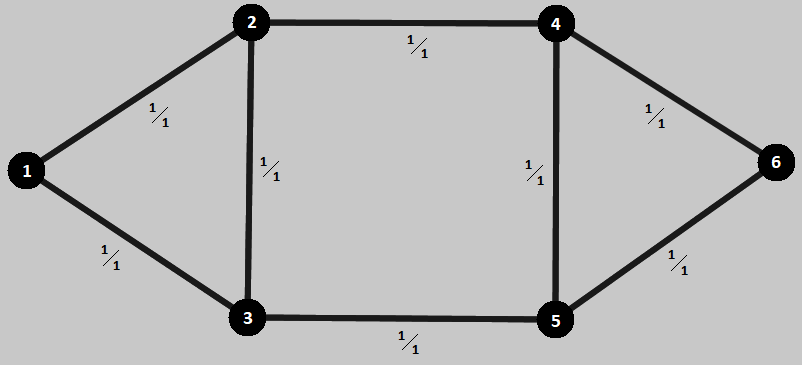
\includegraphics[width=13cm]{sdf/heuristic/figures/topologies/opaque_surv/medium/physical_topology_medium}
\caption{Physical Topology.}
\label{physical_topology_surv_ref_medium_heuristic}
\end{figure}

Following all the steps mentioned in the \ref{net2plan_guide}, applying the routing and grooming heuristic algorithms in the Net2Plan software and using all the data referring to this scenario, the obtained result for the Vasco's heuristics can be consulted in the following table:

\begin{table}[H]
\centering
\begin{tabular}{|| c | c | c | c | c | c | c ||}
 \hline
 \multicolumn{7}{|| c ||}{CAPEX of the Network} \\
 \hline
 \hline
 \multicolumn{3}{|| c |}{ } & Quantity & Unit Price & Cost & Total \\
 \hline
 \multirow{3}{*}{Link Cost} & \multicolumn{2}{ c |}{OLTs} & 16 & 15 000 \euro & 240 000 \euro & \multirow{3}{*}{94 520 000 \euro} \\ \cline{2-6}
 & \multicolumn{2}{ c |}{100 Gb/s Transceivers} & 188 & 5 000 \euro/Gb/s & 94 000 000 \euro & \\ \cline{2-6}
 & \multicolumn{2}{ c |}{Amplifiers} & 70 & 4 000 \euro & 280 000 \euro & \\
 \hline
 \multirow{9}{*}{Node Cost} & \multirow{7}{*}{Electrical} & EXCs & 6 & 10 000 \euro & 60 000 \euro & \multirow{9}{*}{18 885 900 \euro} \\ \cline{3-6}
 & & ODU0 Ports & 600 & 8 \euro/Gb/s & 6 000 \euro & \\ \cline{3-6}
 & & ODU1 Ports & 500 & 6 \euro/Gb/s & 7 500 \euro & \\ \cline{3-6}
 & & ODU2 Ports & 160 & 3 \euro/Gb/s & 4 800 \euro & \\ \cline{3-6}
 & & ODU3 Ports & 60 & 1.5 \euro/Gb/s & 3 600 \euro & \\ \cline{3-6}
 & & ODU4 Ports & 40 & 1 \euro/Gb/s & 4 000 \euro & \\ \cline{3-6}
 & & Line Ports & 188 & 1 000 \euro/Gb/s & 18 800 000 \euro & \\ \cline{2-6}
 & \multirow{2}{*}{Optical} & OXCs & 0 & 20 000 \euro & 0 \euro & \\ \cline{3-6}
 & & Ports & 0 & 2 500 \euro/porto & 0 \euro & \\
 \hline
 \multicolumn{6}{|| c |}{Total Network Cost} & 113 405 900 \euro \\
\hline
\end{tabular}
\caption{Table with detailed description of CAPEX of Vasco's 2016 results.}
\label{scriptopaque_surv_ref_medium_heuristic_Vasco}
\end{table}

Through the formulas mentioned below we can see how all the values of the quantity column were calculated.

\begin{table}[H]
\centering
\begin{tabular}{|| c | c ||}
 \hline
 OLTs: & \(\displaystyle 2 \sum_{i=1}^{N}\sum_{j=i+1}^{N} L_{ij} \) \\ \hline
 Transceivers: & \(\displaystyle 2 \sum_{i=1}^{N}\sum_{j=i+1}^{N} W_{ij} \) \\ \hline
 Amplifiers: & \(\displaystyle \sum_{i=1}^{N}\sum_{j=i+1}^{N} N^R_{ij} L_{ij} \) \\ \hline
 EXCs: & \(\displaystyle \sum_n^N N_{EXC,n} \) \\ \hline
 ODU0: & \(\displaystyle \sum_{o=1}^{N}\sum_{d=1}^{N} D_{od,0} \) \\ \hline
 ODU1: & \(\displaystyle \sum_{o=1}^{N}\sum_{d=1}^{N} D_{od,1} \) \\ \hline
 ODU2: & \(\displaystyle \sum_{o=1}^{N}\sum_{d=1}^{N} D_{od,2} \)\\ \hline
 ODU3: & \(\displaystyle \sum_{o=1}^{N}\sum_{d=1}^{N} D_{od,3} \) \\ \hline
 ODU4: & \(\displaystyle \sum_{o=1}^{N}\sum_{d=1}^{N} D_{od,4} \) \\ \hline
 Line: & \(\displaystyle \sum_{i=1}^{N}\sum_{j=1}^{N} W_{ij} \) \\ \hline
 OXCs: & As mentioned initially this result is always zero. \\ \hline
 Ports: & Does not exist for this case then it is equal to zero. \\
 \hline
 \end{tabular}
\caption{Table with description of calculation}
\label{formulas_opaque_surv_ref_medium_heuristic}
\end{table}

\textbf{High Traffic Scenario:}\\

In this scenario we have to take into account the traffic calculated in \ref{low_traffic_scenario}. In a first phase we will show the various existing topologies of the network. The first are the allowed topologies, physical and optical topology, the second are the logical topology for all ODUs and finally the resulting physical and optical topology.\\

\begin{figure}[H]
\centering
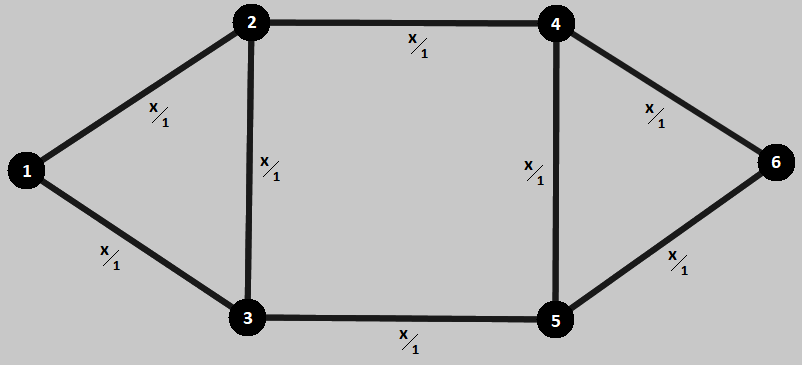
\includegraphics[width=13cm]{sdf/heuristic/figures/topologies/opaque_protec/high/allowed_physical_high}
\caption{Allowed Physical Topology.}
\label{allowed_physical_surv_ref_high_heuristic}
\end{figure}

\begin{figure}[H]
\centering
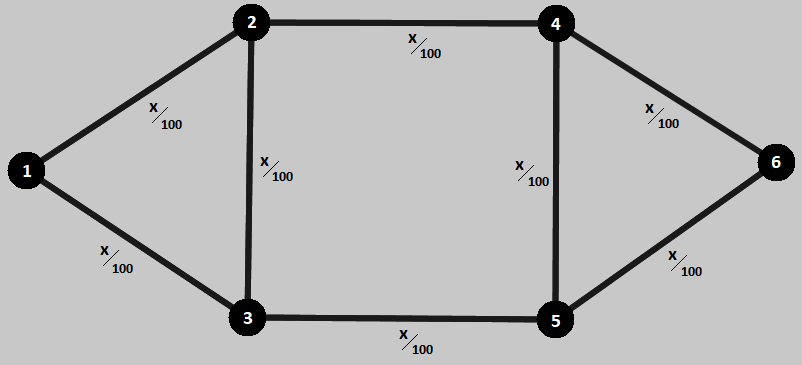
\includegraphics[width=13cm]{sdf/heuristic/figures/topologies/opaque_protec/high/allowed_optical_high}
\caption{Allowed Optical Topology.}
\label{allowed_optical_surv_ref_high_heuristic}
\end{figure}

\begin{figure}[H]
\centering
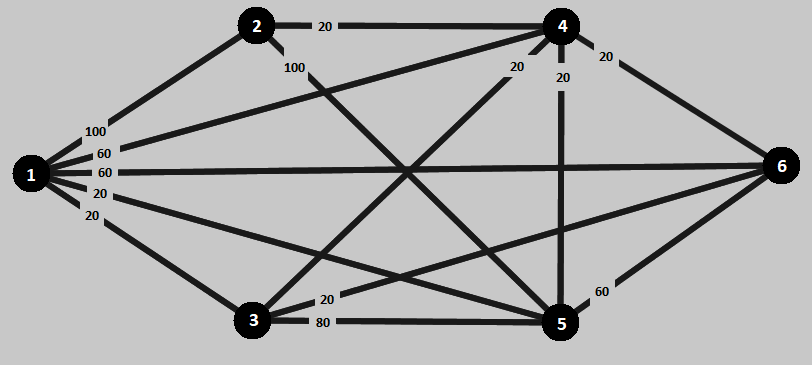
\includegraphics[width=13cm]{sdf/heuristic/figures/topologies/opaque_protec/high/logical_topology_odu0_high}
\caption{Logical Topology of ODU0.}
\label{logical_ODU0_surv_ref_high_heuristic}
\end{figure}

\begin{figure}[H]
\centering
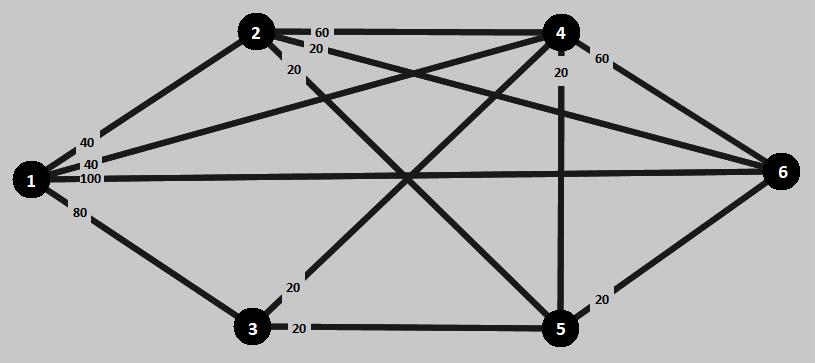
\includegraphics[width=13cm]{sdf/heuristic/figures/topologies/opaque_protec/high/logical_topology_odu1_high}
\caption{Logical Topology of ODU1.}
\label{logical_ODU1_surv_ref_high_heuristic}
\end{figure}

\begin{figure}[H]
\centering
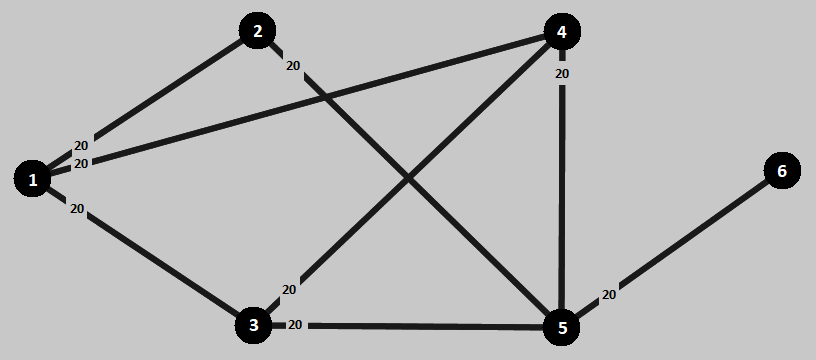
\includegraphics[width=13cm]{sdf/heuristic/figures/topologies/opaque_protec/high/logical_topology_odu2_high}
\caption{Logical Topology of ODU2.}
\label{logical_ODU2_surv_ref_high_heuristic}
\end{figure}

\begin{figure}[H]
\centering
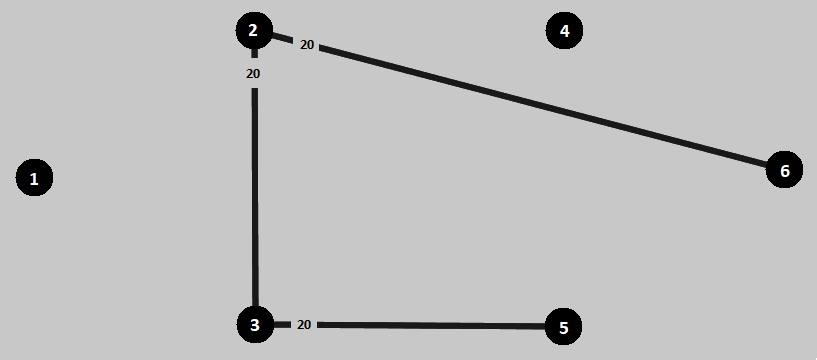
\includegraphics[width=13cm]{sdf/heuristic/figures/topologies/opaque_protec/high/logical_topology_odu3_high}
\caption{Logical Topology of ODU3.}
\label{logical_ODU3_surv_ref_high_heuristic}
\end{figure}

\begin{figure}[H]
\centering
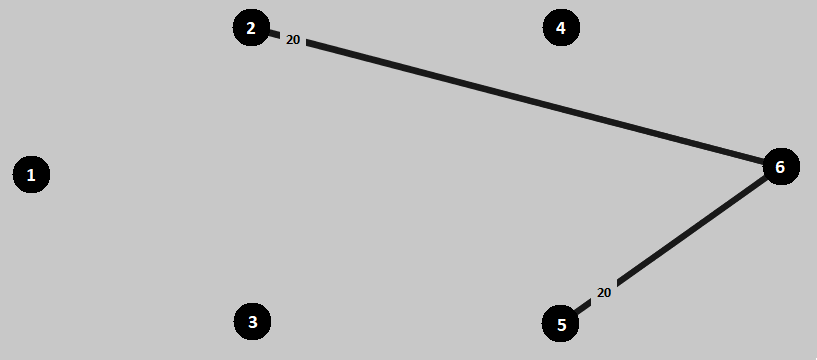
\includegraphics[width=13cm]{sdf/heuristic/figures/topologies/opaque_protec/high/logical_topology_odu4_high}
\caption{Logical Topology of ODU4.}
\label{logical_ODU4_surv_ref_high_heuristic}
\end{figure}

\begin{figure}[H]
\centering
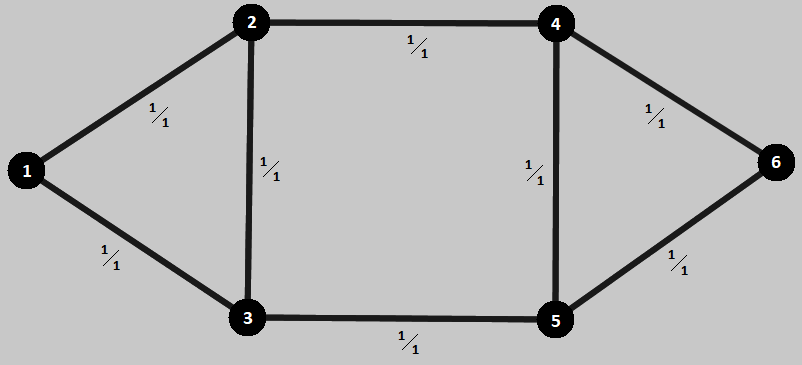
\includegraphics[width=13cm]{sdf/heuristic/figures/topologies/opaque_protec/high/physical_topology_high}
\caption{Physical Topology.}
\label{physical_topology_surv_ref_high_heuristic}
\end{figure}

Following all the steps mentioned in the \ref{net2plan_guide}, applying the routing and grooming heuristic algorithms in the Net2Plan software and using all the data referring to this scenario, the obtained result for the Vasco's heuristics can be consulted in the following table:

\begin{table}[H]
\centering
\begin{tabular}{|| c | c | c | c | c | c | c ||}
 \hline
 \multicolumn{7}{|| c ||}{CAPEX of the Network} \\
 \hline
 \hline
 \multicolumn{3}{|| c |}{ } & Quantity & Unit Price & Cost & Total \\
 \hline
 \multirow{3}{*}{Link Cost} & \multicolumn{2}{ c |}{OLTs} & 16 & 15 000 \euro & 240 000 \euro & \multirow{3}{*}{186 020 000 \euro} \\ \cline{2-6}
 & \multicolumn{2}{ c |}{100 Gb/s Transceivers} & 371 & 5 000 \euro/Gb/s & 185 500 000 \euro & \\ \cline{2-6}
 & \multicolumn{2}{ c |}{Amplifiers} & 70 & 4 000 \euro & 280 000 \euro & \\
 \hline
 \multirow{9}{*}{Node Cost} & \multirow{7}{*}{Electrical} & EXCs & 6 & 10 000 \euro & 60 000 \euro & \multirow{9}{*}{37 211 800 \euro} \\ \cline{3-6}
 & & ODU0 Ports & 1 200 & 8 \euro/Gb/s & 12 000 \euro & \\ \cline{3-6}
 & & ODU1 Ports & 1 000 & 6 \euro/Gb/s & 15 000 \euro & \\ \cline{3-6}
 & & ODU2 Ports & 320 & 3 \euro/Gb/s & 9 600 \euro & \\ \cline{3-6}
 & & ODU3 Ports & 120 & 1.5 \euro/Gb/s & 7 200 \euro & \\ \cline{3-6}
 & & ODU4 Ports & 80 & 1 \euro/Gb/s & 8 000 \euro & \\ \cline{3-6}
 & & Line Ports & 371 & 1 000 \euro/Gb/s & 37 100 000 \euro & \\ \cline{2-6}
 & \multirow{2}{*}{Optical} & OXCs & 0 & 20 000 \euro & 0 \euro & \\ \cline{3-6}
 & & Ports & 0 & 2 500 \euro/porto & 0 \euro & \\
 \hline
 \multicolumn{6}{|| c |}{Total Network Cost} & 223 231 800 \euro \\
\hline
\end{tabular}
\caption{Table with detailed description of CAPEX of Vasco's 2016 results.}
\label{scriptopaque_surv_ref_high_heuristic_Vasco}
\end{table}

Through the formulas mentioned below we can see how all the values of the quantity column were calculated.

\begin{table}[H]
\centering
\begin{tabular}{|| c | c ||}
 \hline
 OLTs: & \(\displaystyle 2 \sum_{i=1}^{N}\sum_{j=i+1}^{N} L_{ij} \) \\ \hline
 Transceivers: & \(\displaystyle 2 \sum_{i=1}^{N}\sum_{j=i+1}^{N} W_{ij} \) \\ \hline
 Amplifiers: & \(\displaystyle \sum_{i=1}^{N}\sum_{j=i+1}^{N} N^R_{ij} L_{ij} \) \\ \hline
 EXCs: & \(\displaystyle \sum_n^N N_{EXC,n} \) \\ \hline
 ODU0: & \(\displaystyle \sum_{o=1}^{N}\sum_{d=1}^{N} D_{od,0} \) \\ \hline
 ODU1: & \(\displaystyle \sum_{o=1}^{N}\sum_{d=1}^{N} D_{od,1} \) \\ \hline
 ODU2: & \(\displaystyle \sum_{o=1}^{N}\sum_{d=1}^{N} D_{od,2} \)\\ \hline
 ODU3: & \(\displaystyle \sum_{o=1}^{N}\sum_{d=1}^{N} D_{od,3} \) \\ \hline
 ODU4: & \(\displaystyle \sum_{o=1}^{N}\sum_{d=1}^{N} D_{od,4} \) \\ \hline
 Line: & \(\displaystyle \sum_{i=1}^{N}\sum_{j=1}^{N} W_{ij} \) \\ \hline
 OXCs: & As mentioned initially this result is always zero. \\ \hline
 Ports: & Does not exist for this case then it is equal to zero. \\
 \hline
 \end{tabular}
\caption{Table with description of calculation}
\label{formulas_opaque_surv_ref_high_heuristic}
\end{table}